\documentclass{article}
\usepackage{graphicx} % Required for inserting images
% header

%% natbib
\usepackage{natbib}
\bibliographystyle{plain}

%% comment
\usepackage{comment}

% no automatic indentation
\usepackage{indentfirst}

% manually indent
\usepackage{xargs} % \newcommandx
\usepackage{calc} % calculation
\newcommandx{\tab}[1][1=1]{\hspace{\fpeval{#1 * 10}pt}}
% \newcommand[number of parameters]{output}
% \newcommandx[number of parameters][parameter index = x]{output}
% use parameter index = x to substitute the default argument
% use #1, #2, ... to get the first, second, ... arguments
% \tab for indentation
% \tab{2} for for indentation twice

% note
\newcommandx{\note}[1]{\textit{\textcolor{red}{#1}}}
\newcommand{\todo}{\note{TODO}}
% \note{TODO}

%% math package
\usepackage{amsfonts}
\usepackage{amsmath}
\usepackage{amssymb}
\usepackage{tikz-cd}
\usepackage{mathtools}
\usepackage{amsthm}

%% operator
\DeclareMathOperator{\tr}{tr}
\DeclareMathOperator{\diag}{diag}
\DeclareMathOperator{\sign}{sign}
\DeclareMathOperator{\grad}{grad}
\DeclareMathOperator{\curl}{curl}
\DeclareMathOperator{\Div}{div}
\DeclareMathOperator{\card}{card}
\DeclareMathOperator{\Span}{span}
\DeclareMathOperator{\real}{Re}
\DeclareMathOperator{\imag}{Im}
\DeclareMathOperator{\supp}{supp}
\DeclareMathOperator{\im}{im}
\DeclareMathOperator{\aut}{Aut}
\DeclareMathOperator{\inn}{Inn}
\DeclareMathOperator{\Char}{char}
\DeclareMathOperator{\Sylow}{Syl}
\DeclareMathOperator{\coker}{coker}
\DeclareMathOperator{\inc}{in}
\DeclareMathOperator{\Sd}{Sd}
\DeclareMathOperator{\Hom}{Hom}
\DeclareMathOperator{\interior}{int}
\DeclareMathOperator{\ob}{ob}
\DeclareMathOperator{\Set}{Set}
\DeclareMathOperator{\Top}{Top}
\DeclareMathOperator{\Meas}{Meas}
\DeclareMathOperator{\Grp}{Grp}
\DeclareMathOperator{\Ab}{Ab}
\DeclareMathOperator{\Ch}{Ch}
\DeclareMathOperator{\Fun}{Fun}
\DeclareMathOperator{\Gr}{Gr}
\DeclareMathOperator{\End}{End}
\DeclareMathOperator{\Ad}{Ad}
\DeclareMathOperator{\ad}{ad}
\DeclareMathOperator{\Bil}{Bil}
\DeclareMathOperator{\Skew}{Skew}
\DeclareMathOperator{\Tor}{Tor}
\DeclareMathOperator{\Ho}{Ho}
\DeclareMathOperator{\RMod}{R-Mod}
\DeclareMathOperator{\Ev}{Ev}
\DeclareMathOperator{\Nat}{Nat}
\DeclareMathOperator{\id}{id}
\DeclareMathOperator{\Var}{Var}
\DeclareMathOperator{\Cov}{Cov}
\DeclareMathOperator{\RV}{RV}
\DeclareMathOperator{\rank}{rank}

%% pair delimiter
\DeclarePairedDelimiter{\abs}{\lvert}{\rvert}
\DeclarePairedDelimiter{\inner}{\langle}{\rangle}
\DeclarePairedDelimiter{\tuple}{(}{)}
\DeclarePairedDelimiter{\bracket}{[}{]}
\DeclarePairedDelimiter{\set}{\{}{\}}
\DeclarePairedDelimiter{\norm}{\lVert}{\rVert}

%% theorems
\newtheorem{axiom}{Axiom}
\newtheorem{definition}{Definition}
\newtheorem{theorem}{Theorem}
\newtheorem{proposition}{Proposition}
\newtheorem{corollary}{Corollary}
\newtheorem{lemma}{Lemma}
\newtheorem{remark}{Remark}
\newtheorem{claim}{Claim}
\newtheorem{problem}{Problem}
\newtheorem{assumption}{Assumption}
\newtheorem{example}{Example}
\newtheorem{exercise}{Exercise}

%% empty set
\let\oldemptyset\emptyset
\let\emptyset\varnothing

\newcommand\eps{\epsilon}

% mathcal symbols
\newcommand\Tau{\mathcal{T}}
\newcommand\Ball{\mathcal{B}}
\newcommand\Sphere{\mathcal{S}}
\newcommand\bigO{\mathcal{O}}
\newcommand\Power{\mathcal{P}}
\newcommand\Str{\mathcal{S}}


% mathbb symbols
\usepackage{mathrsfs}
\newcommand\N{\mathbb{N}}
\newcommand\Z{\mathbb{Z}}
\newcommand\Q{\mathbb{Q}}
\newcommand\R{\mathbb{R}}
\newcommand\C{\mathbb{C}}
\newcommand\F{\mathbb{F}}
\newcommand\T{\mathbb{T}}
\newcommand\Exp{\mathbb{E}}

% mathrsfs symbols
\newcommand\Borel{\mathscr{B}}

% algorithm
\usepackage{algorithm}
\usepackage{algpseudocode}

% longproof
\newenvironment{longproof}[1][\proofname]{%
  \begin{proof}[#1]$ $\par\nobreak\ignorespaces
}{%
  \end{proof}
}


% for (i) enumerate
% \begin{enumerate}[label=(\roman*)]
%   \item First item
%   \item Second item
%   \item Third item
% \end{enumerate}
\usepackage{enumitem}

% insert url by \url{}
\usepackage{hyperref}

% margin
\usepackage{geometry}
\geometry{
a4paper,
total={190mm,257mm},
left=10mm,
top=20mm,
}



\title{ma4261\_hw3}
\author{Nguyen Ngoc Khanh - A0275047B}
\date{August 2024}

\begin{document}

\maketitle

\section{Question 1}
Let $p_{Y|X}$ be a ternary channel with input symbol $\mathcal{X} = \mathcal{Y} = \set{0, 1, 2}$ given by
$$
    P_{Y|X}(y|x) = \begin{cases}
        1 - \eps &\text{if $x = y \neq 1$} \\
        \frac{1-\eps}{2} &\text{if $x=1$ and $y \neq 1$} \\
        \eps &\text{if $y = 1$} \\
        0 &\text{else}
    \end{cases}
$$

\begin{enumerate}[label=(\alph*)]
    \item Draw a diagram with the transition probabilities for this channel
    
    \item Observe any symmetries of this channel. List the permutations $\sigma$ on $\mathcal{X}$ for which there exists a permutation $\sigma'$ on $\mathcal{Y}$ such that $p_{Y|X}(y|x) = p_{Y|X}(\sigma'(y) | \sigma(x))$ for all $x, y$

    \item \label{c} We are interested in the "information channel capacity" $C(p_{Y|X}) = \max_{p_X} I(p_X, P_{Y|X})$. Using the symmetry of the channel, prove that the capacity-achieving input distribution $C(p_{Y|X})$ can be chosen of the following form:
    $$
        p_X^*(x) = \begin{cases}
        \frac{1-q}{2} &\text{if $x \neq 1$} \\
        q &\text{if $x = 1$}
        \end{cases}
    $$

    for some $q \in [0, 1]$ still to be determined.

    \item Using the simplification established in $\ref{c}$ to compute $I(p_X, p_{Y|X})$ as a function of $q$. Determine $C(p_{Y|X})$ and the value $q^*$ that achieves the maximum.

    \item If we fix $q = q^*$, the channel effectively reduces to a well-know channel. Which one?
\end{enumerate}

\subsection{a}

Figure \ref{fig_channel_1a}

\begin{figure}[h]
\centering
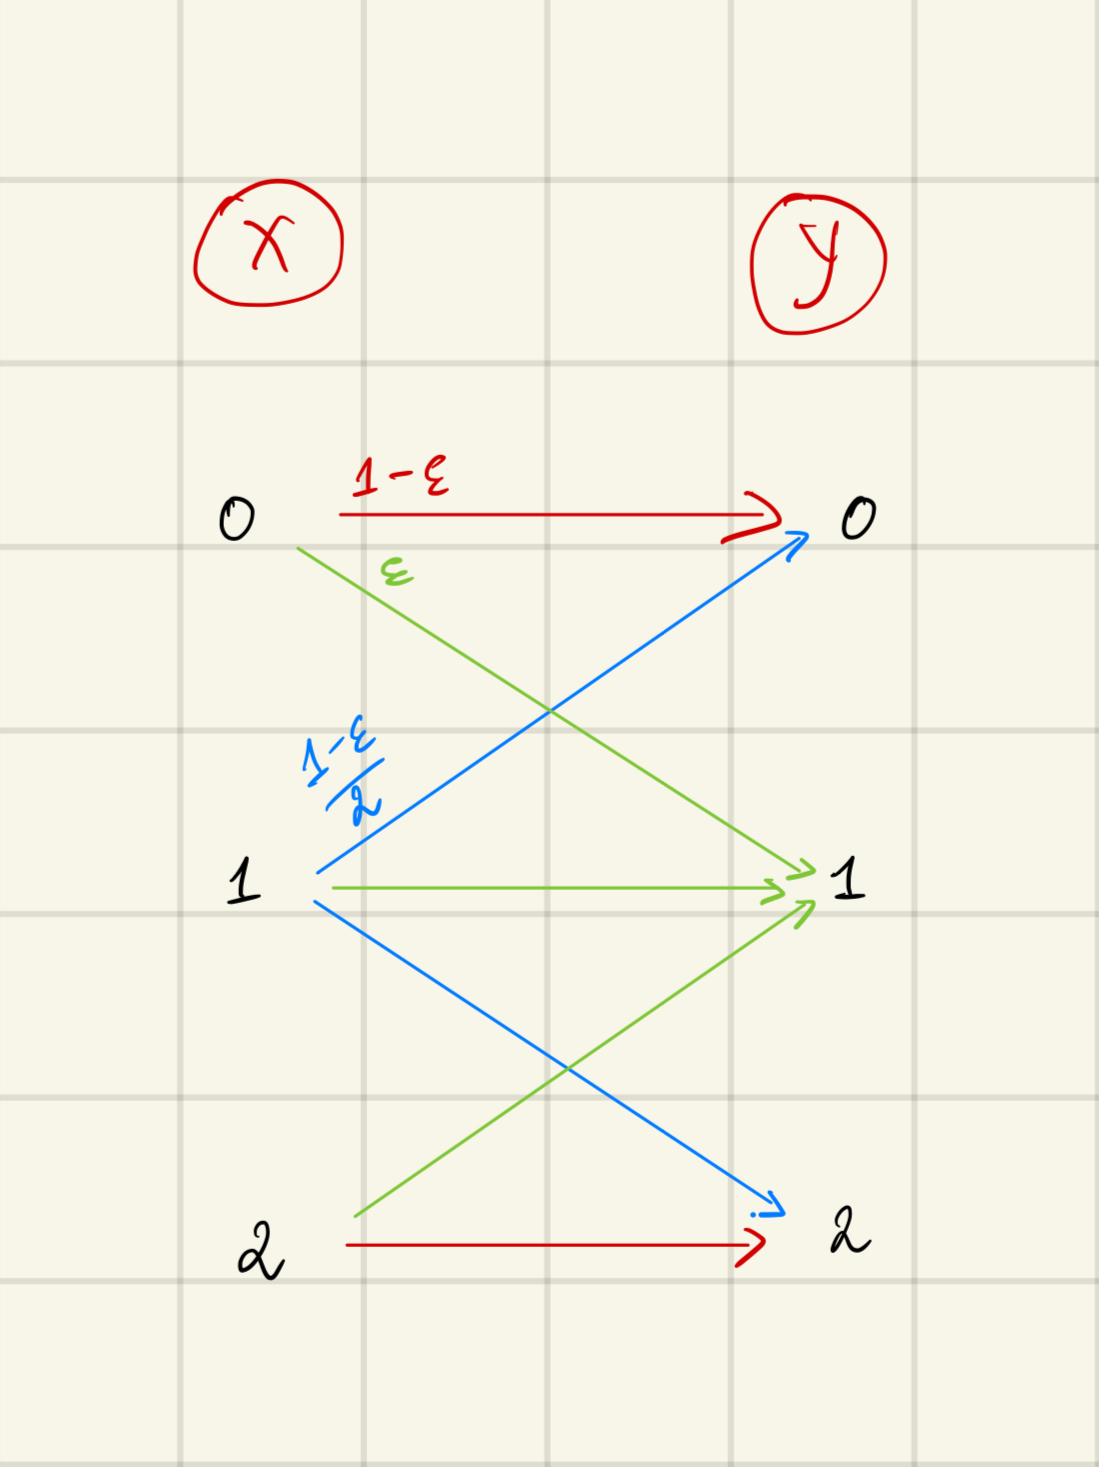
\includegraphics[width=0.5\textwidth]{1a.jpg}
\caption{channel 1a}
\label{fig_channel_1a}
\end{figure}

\subsection{b}

Symmetry of the channel
$$
    \sigma = \sigma' = (2, 1, 0) = \set{(0 \mapsto 2), (2 \mapsto 0)}
$$
\subsection{c}

As $p_X \mapsto I(p_X, p_{Y|X})$ is concave on a convex, compact set, it is either a constant or have exactly one maximum. In both case, if $(0, 1, 2) \mapsto (a, b, c)$ maximizes $I(p_X, p_{Y|X})$, then $(0, 1, 2) \mapsto (c, b, a)$ also maximizes $I(p_X, p_{Y|X})$. Therefore, given $p_X^*$, we must have $p_X^*(0) = p_X^*(2)$. Therefore, $p_X^*$ is of the form
$$
    p_X^*(x) = \begin{cases}
    \frac{1-q}{2} &\text{if $x \neq 1$} \\
    q &\text{if $x = 1$}
    \end{cases}
$$

for $q \in [0, 1]$

\subsection{d}

Let $p_X = p_X^*$. Calculate $p_Y(y)$

\begin{align*}
    p_Y(y)
    &= \sum_{x \in \mathcal{X}} p_{Y|X}(y|x) p_X(x) \\
    &= p_{Y|X}(y|0) p_X(0) + p_{Y|X}(y|1)p_X(1) + p_{Y|X}(y|2)p_X(2) \\
    &= p_{Y|X}(y|0) p_X(0) + p_{Y|X}(y|1)p_X(1) \\
    &= \frac{1-q}{2} p_{Y|X}(y|0) + q p_{Y|X}(y|1) + \frac{1-q}{2} p_{Y|X}(y|2)
\end{align*}

Then
\begin{align*}
    p_Y(0) &= \frac{1-q}{2} (1-\eps) + q \frac{1-\eps}{2} = \frac{1- \eps}{2}\\
    p_Y(1) &= \frac{1-q}{2} \eps + q \eps + \frac{1-q}{2} \eps = \eps\\
    p_Y(2) &= q \frac{1-\eps}{2} + \frac{1-q}{2} (1-\eps) = \frac{1- \eps}{2}
\end{align*}

We have
\begin{align*}
    H(Y)
    &= \sum_{y \in \mathcal{Y}} p_Y(y) \log \frac{1}{p_Y(y)} \\
    &= p_Y(0) \log \frac{1}{p_Y(0)} + p_Y(1) \log \frac{1}{p_Y(1)} + p_Y(2) \log \frac{1}{p_Y(2)} \\
    &= \frac{1 - \eps}{2} \log \frac{2}{1-\eps} + \eps \log \frac{1}{\eps} + \frac{1 - \eps}{2} \log \frac{2}{1-\eps} \\
    &= (1 - \eps) \log \frac{2}{1-\eps} + \eps \log \frac{1}{\eps}
\end{align*}

Let $H_b(\eps)$ denote the entropy of the distribution $[\eps, 1-\eps]$ and $H_t(1/3)$ denote the entropy of the distribution $[1/3, 1/3, 1/3]$

\begin{align*}
    H(Y|X)
    &= \sum_{x \in \mathcal{X}} p_X(x) H(Y | X=x) \\
    &= p_X(0) H(Y | X=0) + p_X(1) H(Y | X=1) + p_X(2) H(Y | X=2) \\
    &= p_X(0) H_b(\eps) + p_X(1) H_t(1/3) + p_X(2) H_b(\eps) \\
    &= (1-q) H_b(\eps) + q H_t(1/3)
\end{align*}

Note that, $H(Y|X)$ is a convex combination of $(H_b(\eps), H_t(1/3))$ that achieves minimum at $\min \set{H_b(\eps), H_t(1/3)}$. As $H_b(\eps) \leq 1 < \log 3 = H_t(1/3)$, therefore, $H(Y|X)$ is minimized at $q^* = 0$. Since, $H(Y)$ is independent of $q$, then $I(X; Y) = H(Y) - H(Y|X)$ is maximized at $q^* = 0$, and the maximum value is

\begin{align*}
    C(p_{Y|X})
    &= H(Y) - H_b(\eps) \\
    &= (1 - \eps) \log \frac{2}{1-\eps} + \eps \log \frac{1}{\eps} - (1 - \eps) \log \frac{1}{1 - \eps} - \eps \log \frac{1}{\eps} \\
    &= 1 - \eps
\end{align*}

\subsection{e}

If we fix $q = q^* = 0$, the channel reduces to binary erasure channel (BEC) of erasing probability $\eps$

\section{Question 2}

Consider the conditional distribution $P_{Y^m | X}$ that stochastically maps $X \in [0, 1]$ to $Y^m \in \set{0, 1}^m$ where given $x \in [0, 1]$, $Y^m$ is i.i.d Bernoulli(x). define the $m$-information channel capacity
$$
    C(m) = \max_{p_X} I(X; Y^m)
$$

We aim to prove, in this question that
$$
    \frac{1}{2} \log m + O(1) \leq C(m) \leq \log m + O(1)
$$

where $O(1)$ is a term that is bounded as $m \to \infty$

\begin{enumerate}[label=(\alph*)]
    \item Let $S = \sum_{i=1}^m Y_i$. Prove that $C(m) = \max_{p_X} I(X, S)$

    \item Let $\Tilde{C}(p_{Y|X}) = \max_{p_X} I (p_X, p_{Y|X})$ be the usual information channel capacity. Prove that
    $$
        \Tilde{C}(p_{Y|X}) = \max_{p_X} \min_{q_Y} D(p_{Y|X} || q_Y|p_X) = \min_{q_Y} \max_{p_X} D(p_{Y|X} || q_Y|p_X)
    $$

    This is known as the saddle point property of the capacity function.

    \item Show using the previous part that
    $$
        C(m) = \min_{q_S} \sup_{x \in [0, 1]} D(Binomial(m, x) || q_S)
    $$

    where $q_S$ is a distribution supported on $\set{0, 1, .., m}$

    \item Choose uniform $q_S$ to show that
    $$
        C(m) \leq \log m + O(1)
    $$

    as $m \to \infty$

    \item Choose uniform $p_X$ to show that for all $\eps > 0$, there exists $m_0(\eps)$ such that for all $m > m_0(\eps)$
    $$
        C(m) \geq \frac{1-\eps}{2} \log m
    $$

\end{enumerate}

Given a Markov chain

\subsection{a}
\begin{center}
\begin{tikzcd}
X \arrow[r] & Y^m \arrow[r] & S(Y)
\end{tikzcd}
\end{center}

As sample mean is a sufficient statistic for Bernoulli RVs, $I(X, Y^m) = I(X, S(Y))$, therefore
$$
    C(m) = \max_{p_X} I(X, Y^m) = \max_{p_X} I(X, S)
$$

\subsection{b}

We have
\begin{align*}
    I(p_X, p_{Y|X})
    &= \sum_{(x, y) \in \mathcal{X} \times \mathcal{Y}} p_{XY}(x, y) \log \frac{p_{XY}(x, y)}{p_X(x) p_Y(y)} \\
    &= \sum_{(x, y) \in \mathcal{X} \times \mathcal{Y}} p_X(x) p_{Y|X}(y | x)  \log \frac{p_{Y|X}(y | x)}{p_Y(y)} \\
    &= \sum_{x \in \mathcal{X}}  p(x) \sum_{y \in \mathcal{Y}} p_{Y|X}(y | x)  \log \frac{p_{Y|X}(y | x)}{p_Y(y)} \\
\end{align*}

Let $q_{Y|X}^*(y | x) = p_Y(y)$ be a conditional probability that is independent of $X$
$$
    I(p_X, p_{Y|X}) = \sum_{x \in \mathcal{X}}  p(x) \sum_{y \in \mathcal{Y}} p_{Y|X}(y | x)  \log \frac{p_{Y|X}(y | x)}{q_{Y|X}^*(y | x)} = D(p_{Y|X} || q_{Y|X}^* | p_X)
$$

Moreover, for any distribution $q_{Y|X}(y | x)$
\begin{align*}
    I(p_X, p_{Y|X})
    &= \sum_{x \in \mathcal{X}}  p(x) \sum_{y \in \mathcal{Y}} p_{Y|X}(y | x)  \log \frac{p_{Y|X}(y | x)}{q_{Y|X}^*(y | x)} \\
    &= \sum_{x \in \mathcal{X}}  p(x) \sum_{y \in \mathcal{Y}} p_{Y|X}(y | x)  \log \frac{p_{Y|X}(y | x)}{q_{Y|X}(y | x)} \frac{q_{Y|X}(y | x)}{q_{Y|X}^*(y | x)} \\
    &= \sum_{x \in \mathcal{X}}  p(x) \sum_{y \in \mathcal{Y}} p_{Y|X}(y | x)  \log \frac{p_{Y|X}(y | x)}{q_{Y|X}(y | x)} + \sum_{x \in \mathcal{X}}  p(x) \sum_{y \in \mathcal{Y}} p_{Y|X}(y | x)  \log \frac{q_{Y|X}(y | x)}{q_{Y|X}^*(y | x)} \\
    &= D(p_{Y|X} || q_{Y|X} | p_X) + \sum_{x \in \mathcal{X}}  p(x) \sum_{y \in \mathcal{Y}} p_{Y|X}(y | x)  \log \frac{q_{Y|X}(y | x)}{q_{Y|X}^*(y | x)} \\
    &= D(p_{Y|X} || q_{Y|X} | p_X) + \sum_{y \in \mathcal{Y}} p_{Y}(y)  \log \frac{q_{Y|X}(y | x)}{q_{Y|X}^*(y | x)} \\
    &= D(p_{Y|X} || q_{Y|X} | p_X) - \sum_{y \in \mathcal{Y}} q_{Y|X}^*(y | x)  \log \frac{q_{Y|X}^*(y | x)}{q_{Y|X}(y | x)} \\
    &= D(p_{Y|X} || q_{Y|X} | p_X) - D(q_{Y|X}^*(\cdot | x) || q_{Y|X}(\cdot | x)) \\
    &\leq D(p_{Y|X} || q_{Y|X} | p_X)
\end{align*}

Therefore, we have

$$
    D(p_{Y|X} || q_{Y|X}^* | p_X) = I(p_X, p_{Y|X}) \leq D(p_{Y|X} || q_{Y|X} | p_X)
$$

Then,
$$
    I(p_X, p_{Y|X}) = \min_{q_{Y|X}} D(p_{Y|X} || q_{Y|X} | p_X)
$$

As $\min_{q_{Y|X}} D(p_{Y|X} || q_{Y|X} | p_X)$ reach its minimum at $q_{Y|X}^* = p_Y$ independent of $X$, therefore,

$$
    I(p_X, p_{Y|X}) = \min_{q_Y} D(p_{Y|X} || q_Y | p_X)
$$

Hence, 
$$
    \Tilde{C}(p_X, p_{Y|X}) = \max_{p_X} \min_{q_{Y|X}} D(p_{Y|X} || q_Y | p_X)
$$

By minimax theorem,

$$
    \Tilde{C}(p_X, p_{Y|X}) = \max_{p_X} \min_{q_Y} D(p_{Y|X} || q_Y | p_X) =  \min_{q_Y} \max_{p_X} D(p_{Y|X} || q_Y | p_X)
$$

\subsection{c}

We have
\begin{align*}
    C(m)
    &= \max_{p_X} I(X, S) \\
    &= \min_{q_{S|X}} \max_{p_X} D(p_{S|X} || q_{S|X} | p_X) \\
    &= \min_{q_{S|X}} \max_{p_X} \int_{x \in [0, 1]} p_X(x) D(p_{S|X}(\cdot | x) || q_{S|X}(\cdot | x)) dx\\
\end{align*}

Note that, the integral $\int_{x \in [0, 1]} p_X(x) D(p_{S|X}(\cdot | x) || q_{S|X}(\cdot | x)) dx$ is maximized when $p_X$ concentrate at one point such that it maximizes $D(p_{S|X}(\cdot | x) || q_{S|X}(\cdot | x))$, therefore
$$
    C(m) = \min_{q_{S|X}} \sup_{x \in [0, 1]} D(p_{S|X}(\cdot | x) || q_{S|X}(\cdot | x))
$$

Given any $x \in [0, 1]$, $p_{S|X}(\cdot | x) = Binomial(m, x)$ and from previous derivations, $q_{S|X}$ independent of $X$ gives the maximum value for $D(p_{S|X}(\cdot | x) || q_{S|X}(\cdot | x))$, then
$$
    C(m) = \min_{q_S} \sup_{x \in [0, 1]} D(Binomial(m, x) || q_S)
$$

\subsection{d}

Let $q_S$ be uniform
\begin{align*}
    D(Binomial(m, x) || q_S)
    &= \sum_{k=0}^m {m \choose k} x^k (1-x)^{n-k} \log \frac{{m \choose k} x^k (1-x)^{n-k}}{1/m} \\
    &= \log m - H(Binomial(m, x)) \leq \log m
\end{align*}
Therefore, 

$$
    C(m) \leq \log m 
$$

for all $m \in \N$. Another proof is that $I(X, S) \leq H(S) \leq \log m$

\subsection{e}
\begin{lemma}
    For any integer-valued random variable $X$ with variance $\sigma^2$, then
    $$
        H(X) \leq \frac{1}{2} \log \bracket*{2 \pi e \tuple*{\sigma^2 + \frac{1}{12}}}
    $$

    Moreover, if $X$ is $Binomial(n, p)$, then $\sigma^2 = np(1-p)$, we have
    $$
        H(X) \leq \frac{1}{2} \log(np(1-p))
    $$
    
\end{lemma}

Main Proof: 
\begin{align*}
    D(Binomial(m, x) || q_S)
    &= \sum_{k=0}^m {m \choose k} x^k (1-x)^{n-k} \log \frac{{m \choose k} x^k (1-x)^{n-k}}{q_S(k)} \\
    &= - H(Binomial(m, x)) + \sum_{k=0}^m {m \choose k} x^k (1-x)^{n-k} \log \frac{1}{q_S(k)} \\
    &\geq - H(Binomial(m, x)) + \log \bracket*{\sum_{k=0}^m {m \choose k} x^k (1-x)^{n-k} \frac{1}{q_S(k)}} &\text{(Jensen)} \\
    &\geq - H(Binomial(m, x)) + \log \bracket*{\sum_{k=0}^m {m \choose k} x^k (1-x)^{n-k}} &\text{($\frac{1}{q_S(k)} \geq 1$)} \\
\end{align*}

\note{TODO - right term is cross entropy}

\section{Question 3}
The problem deals with the converse proof of Shannon's Channel Coding Theorem under the criterion of an "average bit error probability" of decoding

Consider a message $W = (W_1, ... , W_{nR})$ uniformly distributed over $\set{0, 1}^{nR}$, i.e., $W$ consists of $nR$ (treat this as an integer) independent bits $W_1, ... , W_{nR}$. Consider a sequence of ($2nR$, $n$)-codes for the channel with encoder $f_n$ and decoder $\phi_n$. Recall that the average error probability is

$$
    \lambda_{ave} (f_n, \phi_n) = Pr(W \neq \hat{W})
$$

where $\hat{W} = \phi_n(Y^n)$. Denote by $\hat{W}_i$ the estimate of the $i$-th message bit $W_i$ and let 
$$
    b_i(f_n, \phi_n) = Pr(W_i \neq \hat{W}_i)
$$

for $1 \leq i \leq nR$. Furthermore, let the average bit error probability be defined by
$$
    b_{ave}(f_n, \phi_n) = \frac{1}{nR} \sum_{i=1}^{nR} b_i(f_n, \phi_n)
$$

\begin{enumerate}[label=(\alph*)]
    \item Show that $b_{ave}(f_n, \phi_n) \leq \lambda_{ave} (f_n, \phi_n)$

    \item In class we showed the weak converse to Shannon's channel coding theorem which says that under $\lambda_{ave} (f_n, \phi_n) \to 0$, $R \leq C = \max_{p_X} I(p_X, p_{Y|X})$. Show that even if $b_{ave}(f_n, \phi_n) \to 0$, the rate satisfies
    $$
        R \leq C = \max_{p_X} I(p_X, p_{Y|X})
    $$
\end{enumerate}

\subsection{a}

We have

\begin{align*}
    \lambda_{ave} (f_n, \phi_n)
    &= Pr(W \neq \hat{W}) \\
    &= 1 - Pr(W_1 = \hat{W}_1, W_2 = \hat{W}_2, ..., W_{nR} = \hat{W}_{nR}) \\
    &\geq 1 - \min_{i \in [nR]} Pr(W_i = \hat{W}_i) &\text{(monotone)}\\
    &\geq 1 - \frac{1}{nR} \sum_{i=1}^{nR} Pr(W_i = \hat{W}_i) &\text{(minimum is less than average)}\\
    &= \frac{1}{nR} \sum_{i=1}^{nR} \tuple*{1 - Pr(W_i = \hat{W}_i)} \\
    &= \frac{1}{nR} \sum_{i=1}^{nR} Pr(W_i \neq \hat{W}_i) \\
    &= b_{ave}(f_n, \phi_n)
\end{align*}

\subsection{b}

Consider the Markov chain
$$
    (W_1, W_2, ..., W_{nR}) - X^n - Y^n - (\hat{W}_1, \hat{W}_2, ..., \hat{W}_{nR})
$$

Since $W$ is uniformly distributed on $\set{0, 1}^{nR}$, bits are independent, then
$$
    \sum_{i=1}^{nR} I(W_i; \hat{W}_i) \leq I(W; \hat{W})
$$

\begin{align*}
    nC
    &\geq I(X^n; Y^n) \\
    &\geq I(W, \hat{W}) &\text{(DPI)}\\
    &\geq \sum_{i=1}^{nR} I(W_i; \hat{W}_i)
\end{align*}

Let $p_e^i = P(W_i \neq \hat{W}_i)$, note that since $P_{W_i}$ is uniform on $\set{0, 1}$, then
\begin{align*}
    I(W_i; \hat{W}_i)
    &\geq d_b(P_{W_i \hat{W_i}} (W_i = \hat{W}_i), (P_{W_i} \times P_{\hat{W_i}})(W_i = \hat{W}_i)) \\
    &= d_b(1 - p_e^i, 1/2) \\
    &= (1 - p_e^i) \log \frac{1 - p_e^i}{1/2} + p_e^i \log \frac{p_e^i}{1/2} \\
    &= 1 - \log (1 - p_e^i) \\
    &\geq 1 - \frac{1}{\ln 2} p_e^i &\text{(for $p_e^i$ small and positive)}\\
\end{align*}

Then

$$
    nC \geq \sum_{i=1}^{nR} (1 - \frac{1}{\ln 2} p_e^i) 
$$

Then

$$
    C \geq R - R \frac{1}{\ln 2} b_{ave}(f_n, \phi_n)
$$

As $b_{ave}(f_n, \phi_n) \to 0$, we must have $R \leq C$

\section{Question 4} 

[Deterministic Channel] Consider a memoryless channel that takes pairs of bits as input and produces two bits as output as follows: $00 \mapsto 01, 01 \mapsto 10, 10 \mapsto 11, 11 \mapsto 00$. Let $(X_1, X_2)$ denote the two input bits and $(Y_1, Y_2)$ the two output bits

\begin{enumerate}[label=(\alph*)]
    \item Calculate the mutual information $I(X_1, X_2; Y_1, Y_2)$ for a given joint PMF of four pairs of input bits. You can express your answer in terms of
    \begin{align*}
        p_{00} = Pr(X_1 = 0, X_2 = 0) \\
        p_{10} = Pr(X_1 = 1, X_2 = 0) \\
        p_{01} = Pr(X_1 = 0, X_2 = 1) \\
        p_{11} = Pr(X_1 = 1, X_2 = 1)
    \end{align*}

    \item \label{b} Show that the capacity is $2$ and indicate the units of capacity

    \item Show that, surprisingly $I(X_1, Y_1) = 0$ for the capacity-maximizing distribution of the input you derived in part \ref{b}, that is, information is only transferred by considering both bits
\end{enumerate}

\subsection{a}
\begin{align*}
    I(X_1, X_2; Y_1, Y_2)
    &= H(Y_1, Y_2) - H(Y_1, Y_2 | X_1, X_2) \\
    &= H(Y_1, Y_2) &\text{(deterministic)} \\
    &= H(X_1, X_2) &\text{(injective)} \\
    &= \sum_{x_1 x_2 \in \set{00, 01, 10, 11}} p_{x_1 x_2} \log \frac{1}{p_{x_1 x_2}}
\end{align*}

\subsection{b}

$I(X_1, X_2; Y_1, Y_2)$ is maximized when $X_1 X_2$ is uniform, that is
$$
    C = \log \frac{1}{1/4} = 2
$$

\subsection{c}

\begin{align*}
    I(X_1, Y_1)
    &= \sum_{(x, y) \in \set{0, 1}^2} Pr(X_1 = x, Y_1 = y) \log \frac{Pr(X_1 = x, Y_1 = y)}{Pr(X_1 = x) Pr(Y_1 = y)} \\
    &= \sum_{(x, y) \in \set{0, 1}^2} Pr(X_1 = x, Y_1 = y) \log \frac{Pr(Y_1 = y | X_1 = x)}{Pr(Y_1 = y)} \\
\end{align*}

If $X$ is uniform, for every pair $(x, y) \in \set{0, 1}^2$, we always have
$$
    Pr(Y_1 = y | X_1 = x) = Pr(Y_1 = y) = \frac{1}{2}
$$

Therefore, 
$$
    I(X_1, Y_1) = 0
$$

\end{document}
